\documentclass{article}

\usepackage{ipprocess}
%\usepackage{lmodern}
\usepackage{longtable}
\usepackage[utf8]{inputenc} 
\usepackage[T1]{fontenc}
\pagestyle{fancy}
\usepackage{libertine}
\usepackage{epstopdf}
\usepackage{rotating} % rotate table 90 degrees
\usepackage{pdflscape} % set ladscape/portrait pdf pages
\usepackage[table]{xcolor}

%\usepackage[author={João Carlos Nunes Bittencourt}]{pdfcomment}

%%%%
\definecolor{darkred}{rgb}{0.55,0.0,0.0}
%%%%

\sloppy

\title{32-bit $\mu$DLX Core Processor}

\graphicspath{{./pictures/}}
\makeindex
\begin{document}
  \capa{1.0}{july}{2014}{32-bit $\mu$DLX Core Processor}{Verification Plan}{Universidade Federal da Bahia}
  \newpage

%%%%%%%%%%%%%%%%%%%%%%%%%%%%%%%%%%%%%%%%%%%%%%%%%%
%% GNU LGPL Licence
%%%%%%%%%%%%%%%%%%%%%%%%%%%%%%%%%%%%%%%%%%%%%%%%%%

  
\begin{center}
\begin{Large}\textbf{GNU LGPL License}\end{Large}
\end{center}
\vspace{2cm}
\fbox{
  \parbox{.7\textwidth}{
    \vspace{0,5cm}
    \begin{scriptsize}
    This file is part of uDLX (micro-DeLuX) soft IP-core.\\

    uDLX is free soft IP-core: you can redistribute it and/or modify
    it under the terms of the GNU General Public License as published by
    the Free Software Foundation, either version 3 of the License, or
    (at your option) any later version.\\

    uDLX soft core is distributed in the hope that it will be useful,
    but WITHOUT ANY WARRANTY; without even the implied warranty of
    MERCHANTABILITY or FITNESS FOR A PARTICULAR PURPOSE. See the
    GNU General Public License for more details.

    You should have received a copy of the GNU General Public License
    along with uDLX. If not, see <http://www.gnu.org/licenses/>.
    \end{scriptsize}
    \vspace{0,5cm}
  }
}

\newpage

%%%%%%%%%%%%%%%%%%%%%%%%%%%%%%%%%%%%%%%%%%%%%%%%%%
%% Revision History
%%%%%%%%%%%%%%%%%%%%%%%%%%%%%%%%%%%%%%%%%%%%%%%%%%
  \section*{\center Revision History}
  \vspace*{1cm}
  \begin{center} % aqui comeTBDa o ambiente tabela
    \begin{longtable}[pos]{|m{2cm} | m{7.2cm} | m{3.8cm}|} 
      \hline % este comando coloca uma linha na tabela
      \cellcolor[gray]{0.9}
      \textbf{Date} & \cellcolor[gray]{0.9}\textbf{Description} & \cellcolor[gray]{0.9}\textbf{Author(s)}\\ \hline
      \hline
      \small 05/23/2014 & \small First Verification Plan version. & \small Victor Valente \\ \hline
      \small 06/07/2014 & \small Adding information to Overview section. & \small Lauê Rami and Igo Amauri \\ \hline
% Multi-item revision history example
%      \small 05/09/2014 & 
%      \begin{small}
%        \begin{itemize}
%          \item Text revision;
%          \item Update diagrams and instruction layout;
%          \item Update instruction fetch I/O definitions;
%          \item Missing pictures inclusion;
%          \item Include memory access and write back pin/port definitions;
%        \end{itemize}
%      \end{small}  
    \end{longtable}
  \end{center}

  \newpage
	%%%%%%%%%%%%%%%%%%%%%%%%%%%%%%%%%%%%%%%%%%%%%%%%%%	
	%% Place TOC
	%%%%%%%%%%%%%%%%%%%%%%%%%%%%%%%%%%%%%%%%%%%%%%%%%%  
  \tableofcontents
  \newpage

	%%%%%%%%%%%%%%%%%%%%%%%%%%%%%%%%%%%%%%%%%%%%%%%%%%
	%% Document Prelimiary Content
	%%%%%%%%%%%%%%%%%%%%%%%%%%%%%%%%%%%%%%%%%%%%%%%%%%
  \section{Introduction}

	\subsection{Document Purpose}
	The purpose of this document is define the verification plan of the uDLX Implementation. This document includes the 		verification environment used to perform the verification of the processor, beside the main characteristics of the design, the list of tests, list of assertions, and others.
	\subsection{Stakeholders}
  \FloatBarrier
  \begin{table}[H] 
    \begin{center}
      \begin{tabular}[pos]{|m{5cm} | m{8cm}|} 
        \hline % este comando coloca uma linha na tabela
        \cellcolor[gray]{0.9}\textbf{Name} & \cellcolor[gray]{0.9}\textbf{Roles/Responsibilities} \\ \hline
        Igo Amauri Luz & TBD \\ \hline
        Lauê Rami Costa & TBD \\ \hline
      \end{tabular}
    \end{center}
  \end{table} 
  
  \subsection{Document Outline Description}	
  
  \subsection{Acronyms and Abbreviations}
  \FloatBarrier
  \begin{table}[H]
    \begin{center}
      \begin{tabular}[pos]{|m{2cm} | m{11cm}|} 
				\hline 
				\cellcolor[gray]{0.9}\textbf{Acronym} & \cellcolor[gray]{0.9}\textbf{Description} \\ \hline
				ASIC 	& Application Specific Integrated Circuit  \\ \hline
				DUT		& Design Under Test \\ \hline
      \end{tabular}
    \end{center}
  \end{table}  

	%%%%%%%%%%%%%%%%%%%%%%%%%%%%%%%%%%%%%%%%%%%%%%%%%%
	%% Document description
	%%%%%%%%%%%%%%%%%%%%%%%%%%%%%%%%%%%%%%%%%%%%%%%%%%
	\newpage
	\section{DUT Overview}
	The  uDLX is a simplified architecture of the DLX processor. The uDLX correspond to a RISC general propose microprocessor, memory access, arithmetic and logical, and branch instructions. The processor has 5 stages in a pipeline architecture that are : instruction fetch, instruction decode, execute, memory access, and write back.

The uDLX architecture interface is composed by the following components:

	\begin{itemize}
	  \item uDLX 32-bit Core: The core four-deep pipeline processor.
	  \item Memory Interface: Provides a middle layer between the core processor and the external memories. This interface also controls the bootloader process. 
    \item SDRAM Controller: Provides the interface for controlling the external SDRAM.
	\item SRAM Controller: Provides the interface for controlling the external SRAM.
	\end{itemize}

	The Figure \ref{fig:architecture_if} shows the architecture interface.

  \begin{figure}[H]
    \centering
    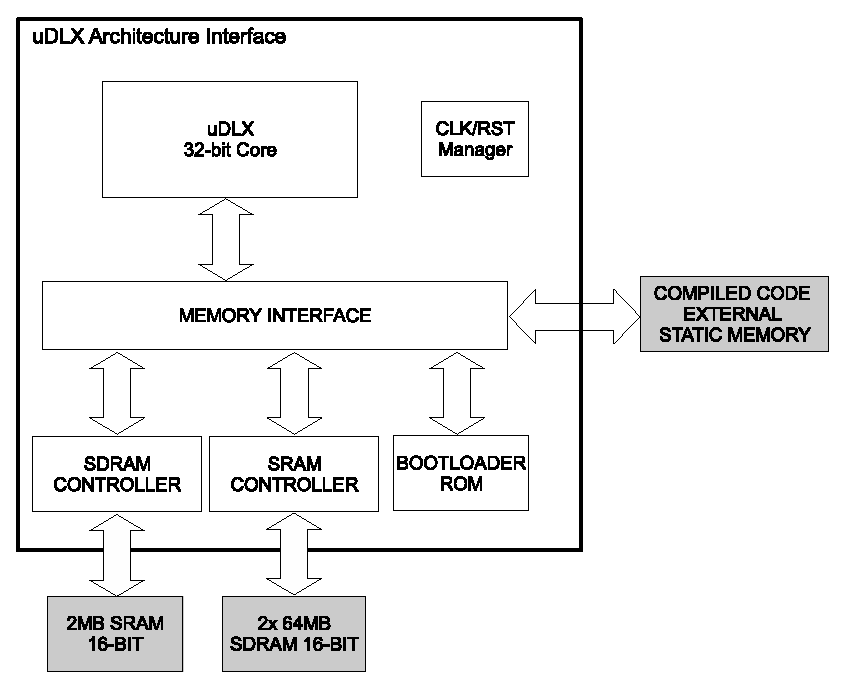
\includegraphics[width=.8\linewidth]{../architecture/pictures/architecture_interface.eps}
    \caption{$\mu$DLX Architecture Interface.}
    \label{fig:architecture_if}    
  \end{figure}	

	A Harvard architecture is implemented using a SRAM with 16 bits of data width to access the instructions and a SDRAM to access data. In order to avoid stall due to time need to access the memories the processor and memories controllers work in different clock rate.

	The main features of the uDLX are:
	\begin{itemize}
		\item uDLX with multiple stages
		\item Hazard handling
		\item SRAM memory access
		\item SDRAM memory access
	\end{itemize}

The Figure \ref{fig:top_architecture} shows the Top Architecture of the $\mu$DLX Processor.	

\begin{landscape}
    \begin{figure}[H]
      \centering
      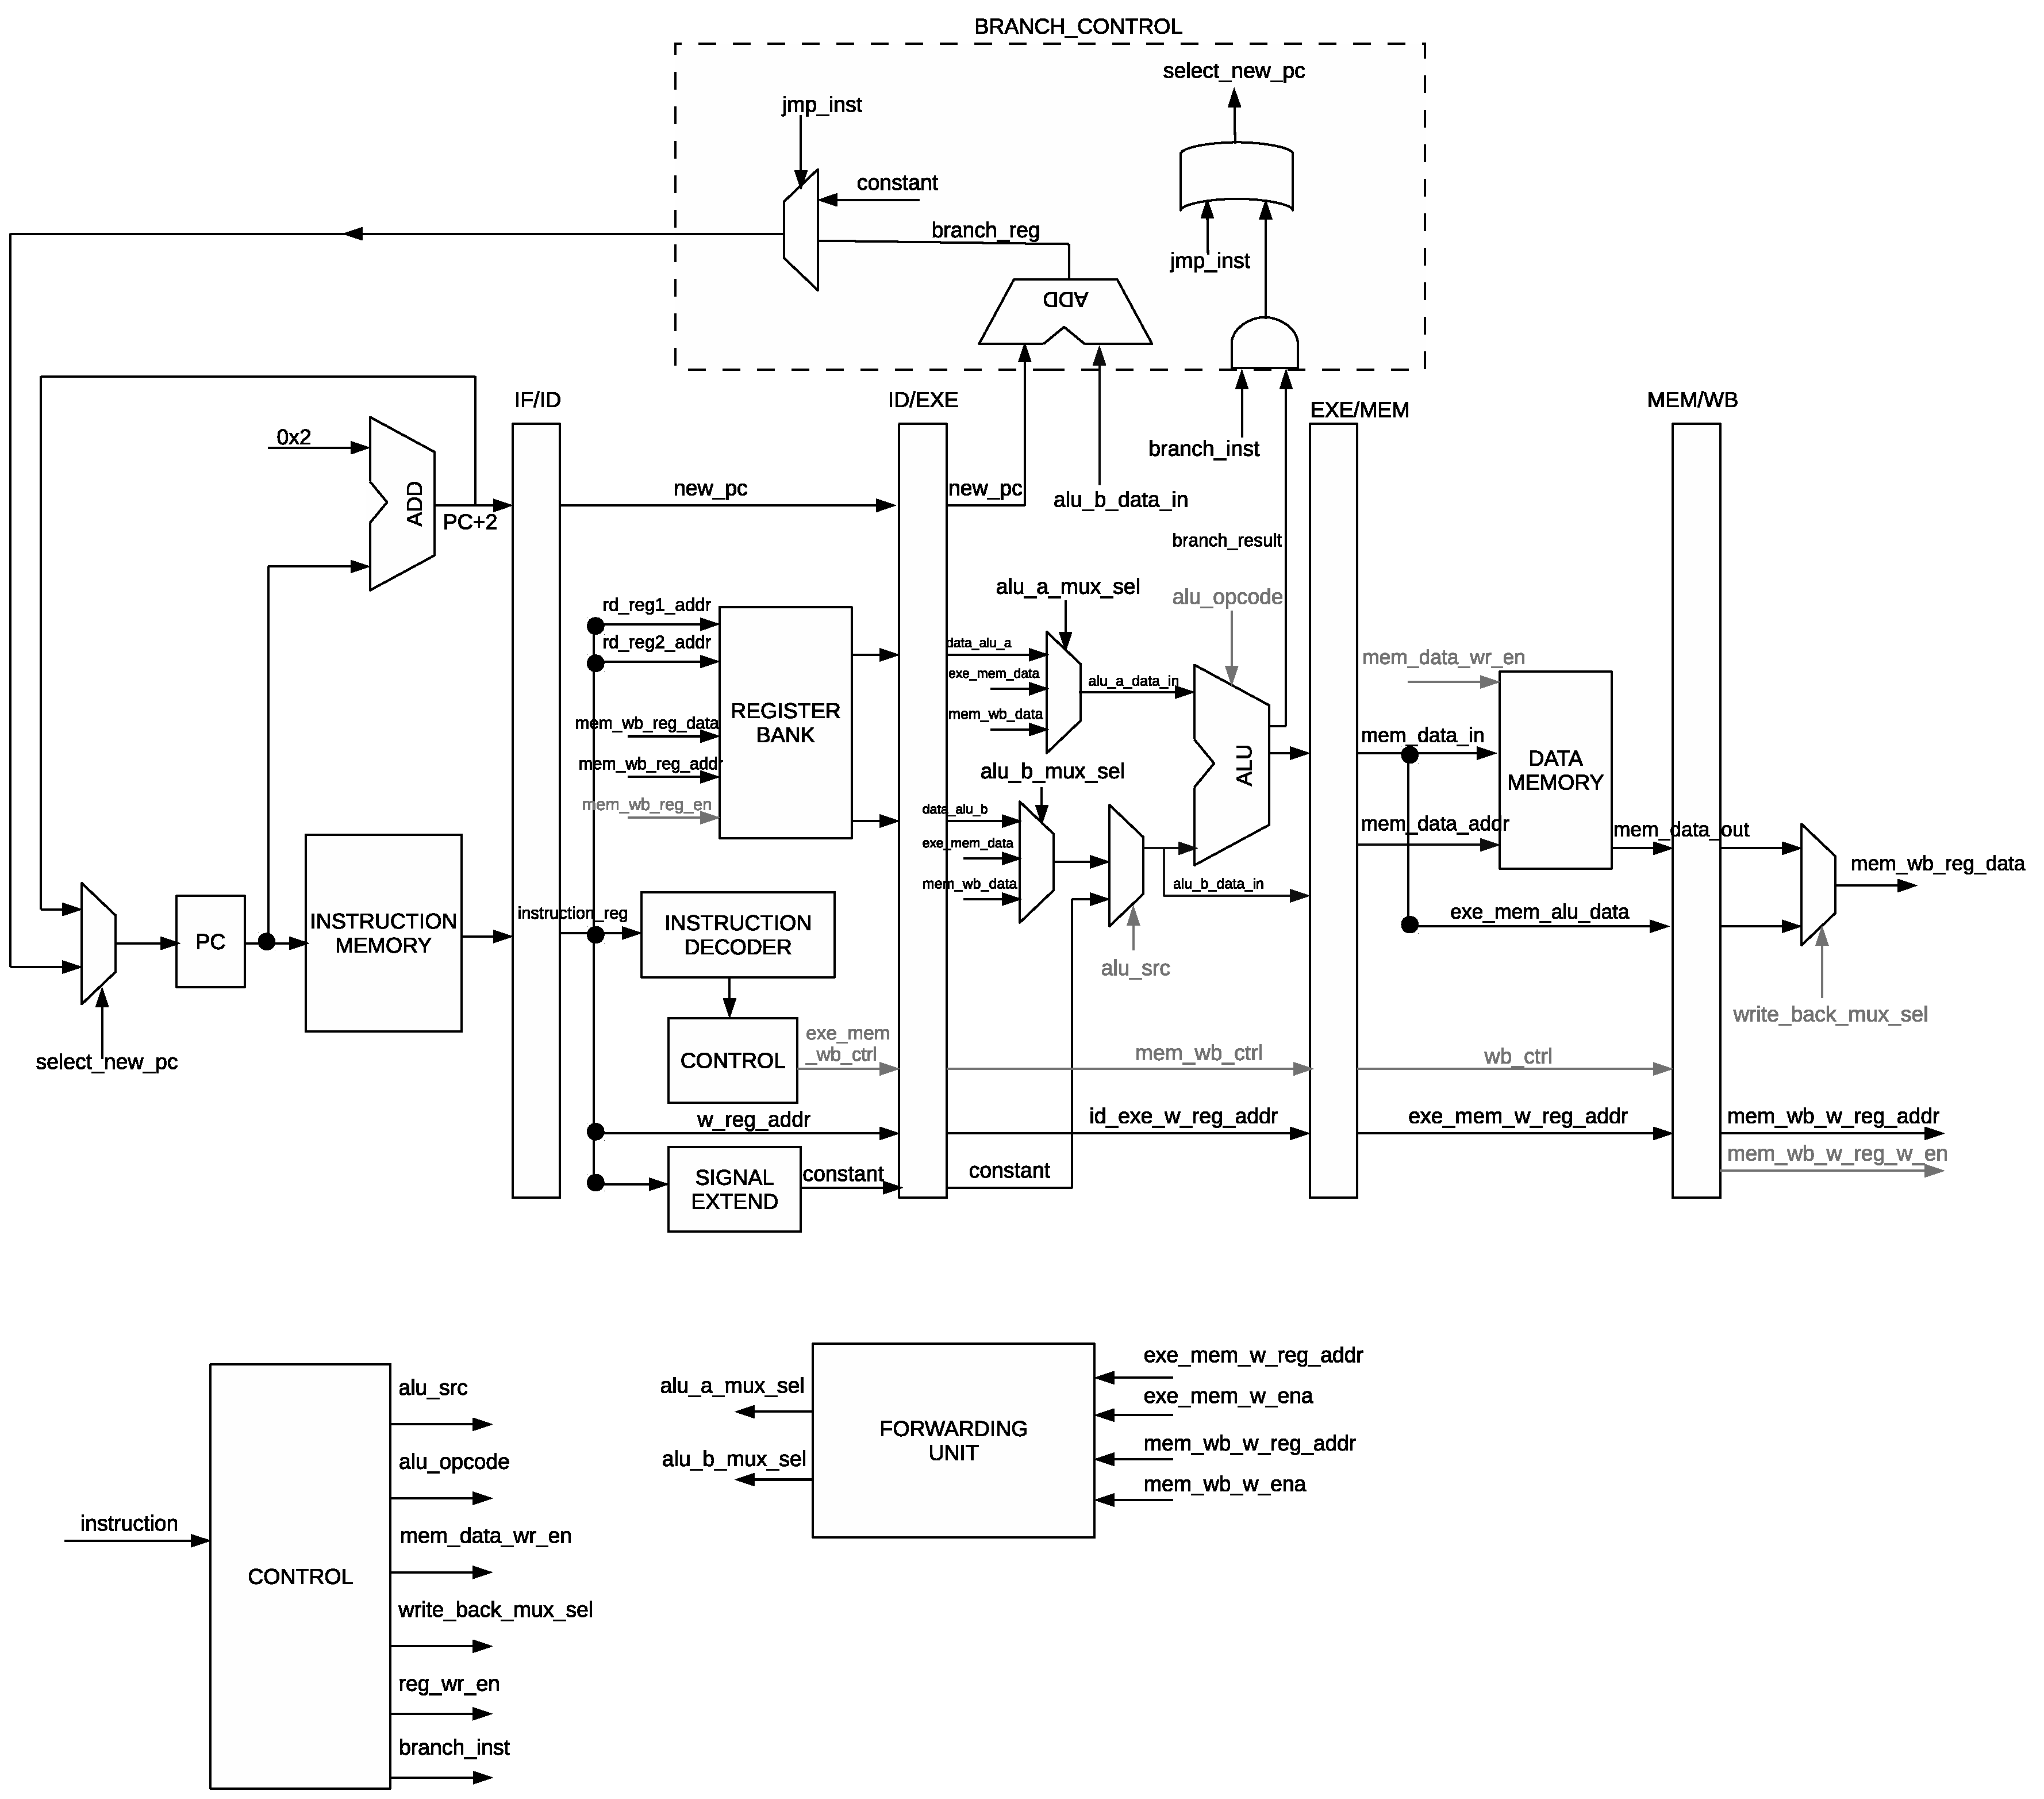
\includegraphics[width=.7\linewidth]{../architecture/pictures/top_architecture.eps}
    	\caption{$\mu$DLX top level architecture overview.}
    	\label{fig:top_architecture}       
    \end{figure}
  \end{landscape}	
	
	In order to be the most close to the DLX and also be as compatible as possible to MIPS R2000 and R3000 architecture few instructions were added to the instruction set of this processor. The instruction set supported in the project are: I-type, R-type and J-type. The Figure \ref{fig:isa} shows the types of instructions.
	
	\begin{figure}[H]
    	\centering
    	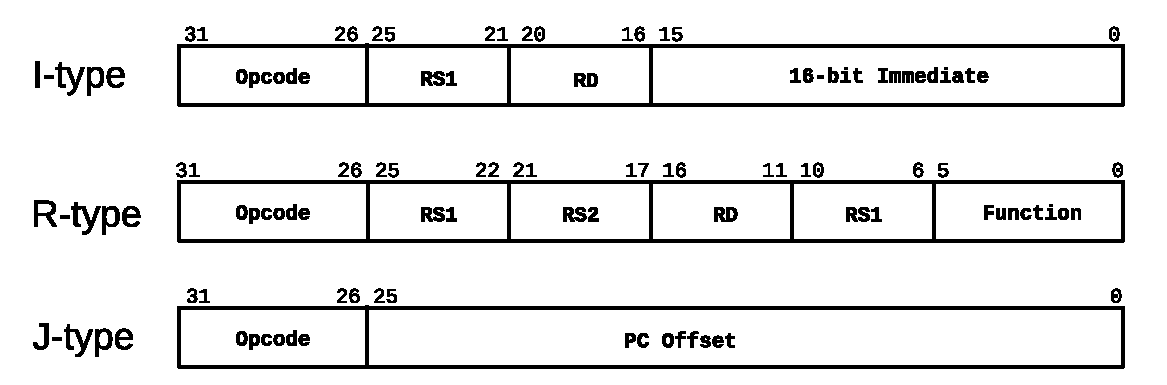
\includegraphics[width=\linewidth]{../architecture/pictures/instruction_set.eps}
    	\caption{$\mu$DLX Instruction Set types definitions.}
    	\label{fig:isa}       	
  	\end{figure} 
  	
	\newpage
	\section{Verification Environment}
	
	The verification methodology is based in a simple testbench. Part of the verification will be done using waveform based verification. Some special situations will be verified using assertion based verification. The design under test (DUT) interface will be responsible to catch data from the uDLX and send to the monitor that will have all assertions. The following topics will describe the items that compose the Verification Plan. The Figure \ref{fig:ver_env} shows the Verification Environment. 
	
		
	\begin{figure}[H]
    	\centering
    	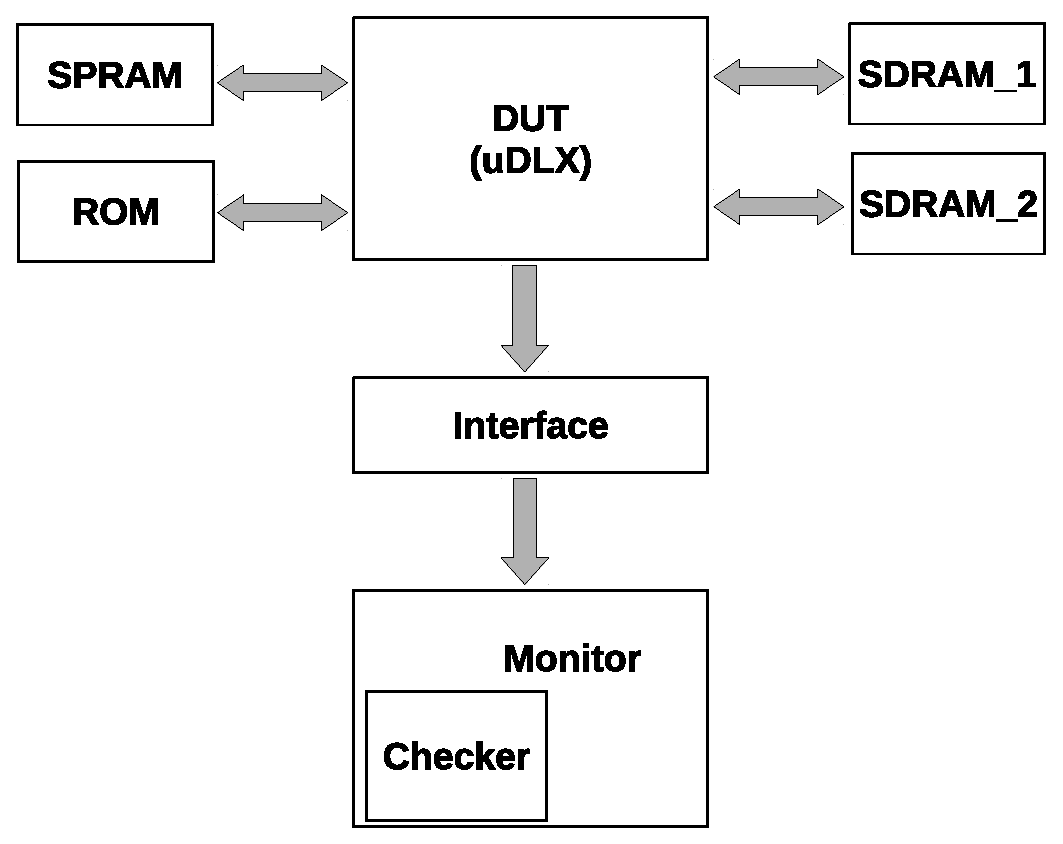
\includegraphics[width=.7\linewidth]{pictures/verification_environment_v2.eps}
    	\caption{$\mu$DLX Verification Environment.}
    	\label{fig:ver_env}
  	\end{figure} 
	
	\subsection{Design Under Test Interface (DUT\_IF)}
	
	The Design Under Test Interface (DUT\_IF) makes the interface between the monitor and the DUT. The DUT\_IF is responsible to control the data that are transmitted between the Verification Environment and DUT, so it contains the instance of all DUT signals that will be used to perform the verification.
	
The DUT Interface, also, have all assertions that is implemented to ensure if the behavior of the DUT signals are correct. 
This interface is instantiated at the Top Level of Verification Environment and the signals are connected with the signals of the DUT.

Through the assertions, the verification ensure, mainly, that the Forwarding, Branch Taken and Load Hazard instructions are working as expected.

	\subsubsection{Forwarding}
	
	The forwarding operation can occur between the execution and different blocks. This assertion will be used to ensure the forwarding unit is activating the correct signal and doing what is expected.
	
	\subsubsection{Branch Taken}
	
	As the uDLX developed work in the branch not taken method, the monitor needs to ensure that when a branch is taken all flush and new address will work correctly.
	
	\subsubsection{Load Hazard}

	During a load hazard the uDLX stall and flush specific stages. The assertions will monitor this condition and give warnings for any unpredicted behavior.	
	
	\subsection{Monitor}
	
	The monitor is responsible to observe the behavior of the DUT and, also, collect the output to verify if the instructions are working as expected.
	
	The monitor observe the behavior of the control signals and, when necessary, capture the data that is stored in data memory and in registers.
	
	When the software ends, the monitor identify it and call the Checker.
The Checker is responsible to execute the Golden Model with the same software that was used by DUT and compare the data stored in data memory and in registers. If any mismatch are found, the errors are reported.

	

	
	\subsection{Verification Environment Design Specification}
  \FloatBarrier
    \begin{center}
			\rowcolors{1}{white}{gray!25}
      \begin{longtable}[pos]{| m{6cm} | m{8cm} |} \hline  
	      \rowcolor{black}
        \multicolumn{1}{|c|}{\textbf{\textcolor{white}{Component}}} & 
        \multicolumn{1}{|c|}{\textbf{\textcolor{white}{Description}}} \\ \hline
        \endfirsthead
        \hline
        \multicolumn{2}{|l|}
        {{\bfseries continued from previous page}} \\
        \hline
        \rowcolor{black}
        \multicolumn{1}{|c|}{\textbf{\textcolor{white}{Component}}} & 
        \multicolumn{1}{|c|}{\textbf{\textcolor{white}{Description}}} \\ \hline
        \endhead
        \hline \multicolumn{2}{|r|}{{continued on next page}} \\ \hline
        \endfoot

        \hline
        \endlastfoot
      	Document Name and Version 		          & $\mu$DLX Verification Plan  	\\ \hline
      	Document Version and Date 		          & Version 1.0, June 23, 2014  	\\ \hline      	
      	Author(s) / Owner(s) 		          			& Lauê Rami / Igo Amauri  	\\ \hline
      	Verification Methodology 		          			& Top-Down  	\\ \hline
      	Verification Methods 		          			& Simulation and Formal Verification  	\\ \hline
      	Simulation Components 		          			&   	\\ \hline
      	Application 		          			& Cadence Incisive  	\\ \hline
      	Languages 		          			& System Verilog  	\\ \hline
      	Verification Environmentv 	&	Custom testbench  \\ \hline	
      	Testbench files				&	At directory: \\ \hline
      	Formal Verification Components	&	Cadence Encounter Conformal \\ \hline
      	Application		&		\\ \hline
      	Technologies	&	FPGA DE2-115  \\ \hline
      \end{longtable}
    \end{center}	
	
	\newpage
	\section{Features List}
	The features list, describes the features that are planned to be implemented.
  \FloatBarrier
    \begin{center}
			\rowcolors{1}{white}{gray!25} 
      \begin{longtable}[pos]{| c | m{9cm} | c |} \hline  %14cm
	      \rowcolor{black}
        \multicolumn{1}{|m{2cm}|}{\centering\textbf{\textcolor{white}{Feature Number}}} & 
        \multicolumn{1}{m{9cm}|}{\centering\textbf{\textcolor{white}{Feature Description}}} &
        \multicolumn{1}{c|}{\textbf{\textcolor{white}{Priority}}}  \\ \hline
        \endfirsthead
        \hline
        \multicolumn{3}{|l|}
        {{\bfseries continued from previous page}} \\
        \hline
        \rowcolor{black}
        \multicolumn{1}{|m{2cm}|}{\centering\textbf{\textcolor{white}{Feature Number}}} & 
        \multicolumn{1}{m{9cm}|}{\textbf{\textcolor{white}{Feature Description}}} &
        \multicolumn{1}{c|}{\textbf{\textcolor{white}{Priority}}}  \\ \hline
        \endhead
        \hline \multicolumn{3}{|r|}{{continued on next page}} \\ \hline
        \endfoot

        \hline
        \endlastfoot
      	DLX\_F1      & Instruction must activate the signals corresponding to the functionality  &	10 \\ \hline   	
      	DLX\_F2      & Forwarding Unit should identify and forward data correctly  &	8 \\ \hline 
      	DLX\_F3      & During a load hazard the stall should work correctly  &	8 \\ \hline
      	DLX\_F4      & Jump hazard should flush before instructions and change PC  &	8 \\ \hline
      	DLX\_F5      & Communication with SRAM must work properly  &	9 \\ \hline
      	DLX\_F6      & Read and write operation to the SDRAM  &	9 \\ \hline
      	DLX\_F7      & The registers of the Register Bank must be reading and writing  &	10 \\ \hline
      	DLX\_F8      & All interfaces protocols must work properly  &	9 \\ \hline     	
      \end{longtable}
    \end{center}	

\begin{landscape}		
	\section{Test List}
	The test list define the tests that will be performed with the DUT to ensure that the behavior is correct. In addition, this tests list ensures achieving coverage levels.
  \FloatBarrier
    \begin{center}
			\rowcolors{1}{white}{gray!25} 
      \begin{longtable}[pos]{| c | m{5cm} | c | c | c | c | c | c |} \hline  %14cm
	      \rowcolor{black}
        \multicolumn{1}{|m{2cm}|}{\centering\textbf{\textcolor{white}{Test \mbox{Number}}}} & 
        \multicolumn{1}{m{5cm}|}{\centering\textbf{\textcolor{white}{Description}}} &
        \multicolumn{1}{c|}{\textbf{\textcolor{white}{Method}}} &
        \multicolumn{1}{c|}{\textbf{\textcolor{white}{Level}}} &
        \multicolumn{1}{m{3cm}|}{\centering\textbf{\textcolor{white}{Features \mbox{Verified}}}} &                
        \multicolumn{1}{c|}{\textbf{\textcolor{white}{Priority}}} & 
        \multicolumn{1}{c|}{\textbf{\textcolor{white}{Owner}}} &
        \multicolumn{1}{c|}{\textbf{\textcolor{white}{Completion}}} \\ \hline
        \endfirsthead
        \hline
        \multicolumn{8}{|l|}
        {{\bfseries continued from previous page}} \\
        \hline
        \rowcolor{black}
        \multicolumn{1}{|m{2cm}|}{\centering\textbf{\textcolor{white}{Test \mbox{Number}}}} & 
        \multicolumn{1}{m{5cm}|}{\centering\textbf{\textcolor{white}{Description}}} &
        \multicolumn{1}{c|}{\textbf{\textcolor{white}{Method}}} &
        \multicolumn{1}{c|}{\textbf{\textcolor{white}{Level}}} &
        \multicolumn{1}{m{3cm}|}{\centering\textbf{\textcolor{white}{Features \mbox{Verified}}}} &                
        \multicolumn{1}{c|}{\textbf{\textcolor{white}{Priority}}} & 
        \multicolumn{1}{c|}{\textbf{\textcolor{white}{Owner}}} &
        \multicolumn{1}{c|}{\textbf{\textcolor{white}{Completion}}} \\ \hline
        \endhead
        \hline \multicolumn{8}{|r|}{{continued on next page}} \\ \hline
        \endfoot

        \hline
        \endlastfoot
      	DLX\_T1      & Execution of all instructions of the Arithmetic category.  &	Sim & Unit & DLX\_F1 & 5 & Lauê & 0\% \\ \hline   
        DLX\_T1\_1    & Execution of addi instruction. All the registers are used to store the results of the operation   &	Sim & Unit & DLX\_F1 & 5 & Lauê & 0\% \\ \hline	
        DLX\_T1\_2    & Execution of subi instruction. All the registers are used to store the results of the operation   &	Sim & Unit & DLX\_F1 & 5 & Lauê & 0\% \\ \hline	
        DLX\_T1\_3    & Execution of add instruction. All the registers are used to store the results of the operation   &	Sim & Unit & DLX\_F1 & 5 & Igo & 0\% \\ \hline	
        DLX\_T1\_4    & Execution of sub instruction. All the registers are used to store the results of the operation   &	Sim & Unit & DLX\_F1 & 5 & Igo & 0\% \\ \hline	
        DLX\_T1\_5    & Execution of cmp instruction. All the registers are used to store the results and a lot of combinations of sources registers are used to perform the comparison   &	Sim & Unit & DLX\_F1 & 5 & Lauê & 0\% \\ \hline
        DLX\_T1\_6    & Execution of not instruction. All the registers are used to store the results and a lot of combinations of sources registers are used to perform the operation   &	Sim & Unit & DLX\_F1 & 5 & Lauê & 0\% \\ \hline
      	DLX\_T2      & Execution of all instructions of the Data Transfer category.  &	Sim & Unit & DLX\_F1 & 5 & Lauê & 0\% \\ \hline   
        DLX\_T2\_1    & Execution of sw instruction. Store determined value in all positions of memory   &	Sim & Unit & DLX\_F1 & 5 & Lauê & 0\% \\ \hline
        DLX\_T2\_2    & Execution of lw instruction. Load the values previously stored in all positions of memory   &	Sim & Unit & DLX\_F1 & 5 & Lauê & 0\% \\ \hline
      	DLX\_T3      & Execution of all instructions of the Logical category.   &	Sim & Unit & DLX\_F1 & 5 & Lauê & 0\% \\ \hline  
        DLX\_T3\_1    & Execution of andi instruction. All the registers are used to store the results of the operation   &	Sim & Unit & DLX\_F1 & 5 & Lauê & 0\% \\ \hline	
        DLX\_T3\_2    & Execution of ori instruction. All the registers are used to store the results of the operation   &	Sim & Unit & DLX\_F1 & 5 & Lauê & 0\% \\ \hline	
        DLX\_T3\_3    & Execution of and instruction. All the registers are used to store the results of the operations   &	Sim & Unit & DLX\_F1 & 5 & Igo & 0\% \\ \hline	
         DLX\_T3\_4    & Execution of or instruction. All the registers are used to store the results of the operations   &	Sim & Unit & DLX\_F1 & 5 & Igo & 0\% \\ \hline

      	DLX\_T4      & Execution of all instructions of the Conditional Branch category.   &	Sim & Unit & DLX\_F1 & 5 & Lauê & 0\% \\ \hline 
      	DLX\_T4\_1   & Execution of beqz instruction. Execute a software that have beqz instruction, and, at least, the condition is satisfied and not.   &	Sim & Unit & DLX\_F1 & 5 & Lauê & 0\% \\ \hline   
      	DLX\_T4\_2   & Execution of bnez instruction. Execute a software that have bnez instruction, and, at least, the condition is satisfied and not.   &	Sim & Unit & DLX\_F1 & 5 & Lauê & 0\% \\ \hline   
      	DLX\_T5      & Execution of all instructions of the Unconditional Jump category.  &	Sim & Unit & DLX\_F1 & 5 & Lauê & 0\% \\ \hline 
       	DLX\_T5\_1   & Execution of jr instruction. Execute a software that have jr instructions and use more than one register as source.   &	Sim & Unit & DLX\_F1 & 5 & Igo & 0\% \\ \hline   
       	DLX\_T5\_2   & Execution of jpc instruction.  &	Sim & Unit & DLX\_F1 & 5 & Igo & 0\% \\ \hline   
	DLX\_T6      & Test forwarding unit in all possible situations  &	Sim & Unit & DLX\_F1, DLX\_F2 & 5 & Igo & 0\% \\ \hline   
	DLX\_T7      & Test the load hazard  &	Sim & Unit & DLX\_F1, DLX\_F3 & 4 & Igo & 0\% \\ \hline   
	DLX\_T8      & Test the SDRAM access  &	Assertion & Unit & DLX\_F6 & 7 & Lauê & 0\% \\ \hline        
	DLX\_T9      & Test the SRAM access  &	Assertion & Unit & DLX\_F5 & 9 & Lauê & 0\% \\ \hline        
	DLX\_T10      & Run programs with the complete architecture  &	Sim & Unit & DLX\_F5, DLX\_F6 & 8 & Igo & 0\% \\ \hline        
	DLX\_T11      & Test All interfaces protocols  & Assertion & Unit & DLX\_F8 & 8 & Igo & 0\% \\ \hline        

      \end{longtable}
    \end{center}		
  \end{landscape}
  
  \newpage
	\section{Assertions}
	Assertion will be used to verify the instructions, specially the instructions that have stall, forwarding and flush.
  \FloatBarrier
    \begin{center}
			\rowcolors{1}{white}{gray!25} 
      \begin{longtable}[pos]{| c | l | c |} \hline  %14cm
	      \rowcolor{black}
        \multicolumn{1}{|c|}{\textbf{\textcolor{white}{Date}}} & 
        \multicolumn{1}{m{9cm}|}{\centering\textbf{\textcolor{white}{Criteria}}} &
        \multicolumn{1}{c|}{\textbf{\textcolor{white}{Status}}}  \\ \hline
        \endfirsthead
        \hline
        \multicolumn{3}{|l|}
        {{\bfseries continued from previous page}} \\
        \hline
        \rowcolor{black}
        \multicolumn{1}{|c|}{\textbf{\textcolor{white}{Date}}} & 
        \multicolumn{1}{m{9cm}|}{\centering\textbf{\textcolor{white}{Criteria}}} &
        \multicolumn{1}{c|}{\textbf{\textcolor{white}{Status}}}  \\ \hline
        \endhead
        \hline \multicolumn{3}{|r|}{{continued on next page}} \\ \hline
        \endfoot

        \hline
        \endlastfoot
      	06/25/2014      & Assertion to the correct fecth\_top operation  &	Not started yet \\ \hline   	
      	06/25/2014      & Assertion to verify the decode operation 			 &	Not started yet \\ \hline
      	07/02/2014      & Assertion for the execution block operation 			 &	Not started yet \\ \hline      	
      	07/02/2014      & Assertion for the memory read and write back 			 &	Not started yet \\ \hline      	
      	07/02/2014      & Assertion to forwarding operation 			 &	Not started yet \\ \hline      	
      	07/02/2014      & Assertion during branches and jumps 			 &	Not started yet \\ \hline      	
      	07/02/2014      & Assertion during load hazard 			 &	Not started yet \\ \hline
      	07/02/2014      & Assertion to verify interfaces protocols 			 &	Not started yet \\ \hline      	
      	
      \end{longtable}
    \end{center}		
	
	\newpage
	\section{Coverage and Completion Requirements}
  \FloatBarrier
    \begin{center}
			\rowcolors{1}{white}{gray!25} 
      \begin{longtable}[pos]{| c | l | c | c | c |} \hline  %14cm
	      \rowcolor{black}
        \multicolumn{1}{|c|}{\textbf{\textcolor{white}{Date}}} & 
        \multicolumn{1}{m{4cm}|}{\centering\textbf{\textcolor{white}{Criteria}}} &
        \multicolumn{1}{m{2cm}|}{\centering\textbf{\textcolor{white}{Required Level}}} &
        \multicolumn{1}{m{2cm}|}{\centering\textbf{\textcolor{white}{Current Level}}} &
        \multicolumn{1}{c|}{\textbf{\textcolor{white}{Status}}} \\ \hline
        \endfirsthead
        \hline
        \multicolumn{5}{|l|}
        {{\bfseries continued from previous page}} \\
        \hline
        \rowcolor{black}
        \multicolumn{1}{|c|}{\textbf{\textcolor{white}{Date}}} & 
        \multicolumn{1}{m{4cm}|}{\centering\textbf{\textcolor{white}{Criteria}}} &
        \multicolumn{1}{m{2cm}|}{\centering\textbf{\textcolor{white}{Required Level}}} &
        \multicolumn{1}{m{2cm}|}{\centering\textbf{\textcolor{white}{Current Level}}} &
        \multicolumn{1}{c|}{\textbf{\textcolor{white}{Status}}} \\ \hline
        \endhead
        \hline \multicolumn{5}{|r|}{{continued on next page}} \\ \hline
        \endfoot

        \hline
        \endlastfoot
      	06/25/2014      & Block coverage  				&	98\% & 0\% & Not started yet \\ \hline   	
      	06/25/2014      & Expression coverage 	 	&	95\% & 0\% & Not started yet \\ \hline      	
      	06/25/2014      & Toggle coverage 	 	&	90\% & 0\% & Not started yet \\ \hline      	
      	06/25/2014      & Code coverage 	 	&	95\% & 0\% & Not started yet \\ \hline      	
      	06/25/2014      & State coverage on FSM 	 	&	100\% & 0\% & Not started yet \\ \hline      	
      	06/25/2014      & Arc coverage on FSM 	 	&	100\% & 0\% & Not started yet \\ \hline      	
      	06/25/2014      & Functional coverage 	 	&	100\% & 0\% & Not started yet \\ \hline      	
      	06/25/2014      & Bug report rate for SPI 	 	&	< 1 bug/day & - & Not started yet \\ \hline      	

      \end{longtable}
    \end{center}	
  
  \newpage
	\section{Resource Requirements}
  \FloatBarrier
    \begin{center}
			\rowcolors{4}{gray!25}{white} 
      \begin{longtable}[pos]{| l | c | c | c | c |} \hline  %14cm
	      \rowcolor{black}
        \multicolumn{1}{|c|}{\textbf{\textcolor{white}{Resource}}} & 
        \multicolumn{1}{c|}{\centering\textbf{\textcolor{white}{Quantity}}} &
        \multicolumn{1}{c|}{\centering\textbf{\textcolor{white}{Description}}} &
        \multicolumn{1}{c|}{\centering\textbf{\textcolor{white}{Start}}} &
        \multicolumn{1}{c|}{\textbf{\textcolor{white}{Duration}}} \\ \hline
        \endfirsthead
        \hline
        \multicolumn{5}{|l|}
        {{\bfseries continued from previous page}} \\
        \hline
        \rowcolor{black}
        \multicolumn{1}{|c|}{\textbf{\textcolor{white}{Resource}}} & 
        \multicolumn{1}{c|}{\centering\textbf{\textcolor{white}{Quantity}}} &
        \multicolumn{1}{c|}{\centering\textbf{\textcolor{white}{Description}}} &
        \multicolumn{1}{c|}{\centering\textbf{\textcolor{white}{Start}}} &
        \multicolumn{1}{c|}{\textbf{\textcolor{white}{Duration}}} \\ \hline
        \endhead
        \hline \multicolumn{5}{|r|}{{continued on next page}} \\ \hline
        \endfoot

        \hline
        \endlastfoot
        \rowcolor{gray}
				\textbf{Engineering Resources}      & 		&										 	& 		 			&  \\ \hline   	
      	Verification Engineer      					& 2		&	1 year experience 	& 06/25/14 	& 10 days \\ \hline   
      	\rowcolor{gray}
				\textbf{Compute Resources}     			& 		&										 	& 		 			&  \\ \hline   
				Computer 														& 1		& 										& 06/25/14	& 10 days \\ \hline   
      	\rowcolor{gray}
				\textbf{Software Resources} 				& 		&										 	& 		 			&  \\ \hline   
				Candence Incisive 									& 1		& 										& 06/25/14	& 10 days \\ \hline 	
				ALTERA Quartus 											& 1		& WEB Edition										& 06/25/14	& 10 days \\ \hline 				
				ALTERA ModelSIM		 									& 1		& WEB Edition										& 06/25/14	& 10 days \\ \hline 
      \end{longtable}
    \end{center}		
  
  \newpage
	\section{Schedule}
  \FloatBarrier
    \begin{center}
			\rowcolors{4}{gray!25}{white} 
      \begin{longtable}[pos]{| l | c | c | m{5.4cm} | m{2cm} |} \hline  %14cm
	      \rowcolor{black}
        \multicolumn{1}{|c|}{\textbf{\textcolor{white}{Resource}}} & 
        \multicolumn{1}{c|}{\centering\textbf{\textcolor{white}{Start}}} &
        \multicolumn{1}{c|}{\centering\textbf{\textcolor{white}{Duration}}} &
        \multicolumn{1}{m{5.4cm}|}{\centering\textbf{\textcolor{white}{Action}}} &
        \multicolumn{1}{m{2cm}|}{\centering\textbf{\textcolor{white}{Compute \mbox{Resource}}}} \\ \hline
        \endfirsthead
        \hline
        \multicolumn{5}{|l|}
        {{\bfseries continued from previous page}} \\
        \hline
        \rowcolor{black}
        \multicolumn{1}{|c|}{\textbf{\textcolor{white}{Resource}}} & 
        \multicolumn{1}{c|}{\centering\textbf{\textcolor{white}{Start}}} &
        \multicolumn{1}{c|}{\centering\textbf{\textcolor{white}{Duration}}} &
        \multicolumn{1}{m{5.4cm}|}{\centering\textbf{\textcolor{white}{Action}}} &
        \multicolumn{1}{m{2cm}|}{\centering\textbf{\textcolor{white}{Compute \mbox{Resource}}}} \\ \hline
        \endhead
        \hline \multicolumn{5}{|r|}{{continued on next page}} \\ \hline
        \endfoot

        \hline
        \endlastfoot
      	Lauê Rami      					& 06/20/14	&	2 Days 	& Develop Verification Test Plan 	& N/A \\ \hline
      	Igo Amauri      					& 06/22/14	&	1 Day 	& Review \& Approve Test Plan 	& N/A \\ \hline
      	Lauê Rami      					& 06/25/14	&	5 Days 	& Create Verification Environment 	& Server 1 \\ \hline
      	Igo Amauri      					& 06/28/14	&	3 Days 	& Features F1,F2,F3, and F4 Verification 	& Server 1 \\ \hline
      	Igo Amauri      					& 07/02/14	&	4 Days 	& Add assertion and code coverage 	& Server 1 \\ \hline
      	Lauê Rami      					& 07/10/14	&	2 Days 	& Complete System simulation and functional verification 	& Server 1 \\ \hline


      \end{longtable}
    \end{center}	
		
	

\end{document}

